% =====================================================================
%  Chapter 20 — The Posterior over the Edge
% =====================================================================

\chapter{The Posterior over the Edge}
\label{ch:posterior-edge}

The phrase ``the edge'' is used loosely in this literature, and the
looseness has done a great deal of damage. This chapter defines it
precisely, shows what the book's model actually produces, and states the
one fact about it that governs the design of everything downstream.

\section{What the edge is, and what it is not}

An edge is a difference between an expected return and a benchmark. It is
not a return. It is not a Sharpe ratio. It is not a t-statistic. It is not
a thing you can observe.

What can be observed, from data, is a posterior distribution over the
edge. The model produces, for each fund and each date, a mean \(\mu\) and
a variance \(v\), and the interpretation is: given everything the model
knows and everything it does not, the expected forward return of this fund
is a random variable with that distribution.

The edge relative to the benchmark is then the difference of two such
random variables, and if the benchmark's own uncertainty is ignored --- as
the book does, since the benchmark is observed rather than estimated ---
the edge has mean \(\mu_i - \mu_b\) and variance \(v_i + v_b\) under
independence.

\section{Why the uncertainty is the product}

Here is the fact that governs the rest of the book, and it is a
straightforward consequence of the definition.

The probability that the edge is actually positive is
\begin{equation}
P(\mu_i - \mu_b > 0) = \Phi\!\left(\frac{\mu_i - \mu_b}
                                        {\sqrt{v_i + v_b}}\right),
\end{equation}
where \(\Phi\) is the standard normal cumulative distribution function.
The book computes it, and it is the number that drives everything.

If the posterior mean of the edge is smaller than the posterior standard
deviation of the edge --- which, given that the model's forecasts are
small relative to their uncertainty, is the normal case --- then the
probability that the edge is positive is close to one half. There is no
evidence. And a system that trades on a coin-flip-sized edge, with the
same position size it would use for a well-established premium, will
lose the spread on every one of those trades.

\begin{takeaway}[The governing fact]
A forecast of magnitude \(\mu\) with uncertainty \(v\) is evidence of a
positive edge only when \(\mu \gg \sqrt{v}\). Until then the honest
statement is that the model does not know, and the only rational response
to not knowing is to hold the position one would hold without the model.
\end{takeaway}

This is the point at which the book's architecture and the literature's
usual architecture diverge. A conventional machine-learning pipeline
trains a model, produces a ranking, holds the top \(k\) names, and
reports the backtest. Every step of that pipeline assumes that the
ranking is informative. The book's pipeline produces a ranking \emph{and}
a probability that the ranking is informative, and the second number
controls the size of the first.

\begin{figure}[!htbp]
\centering
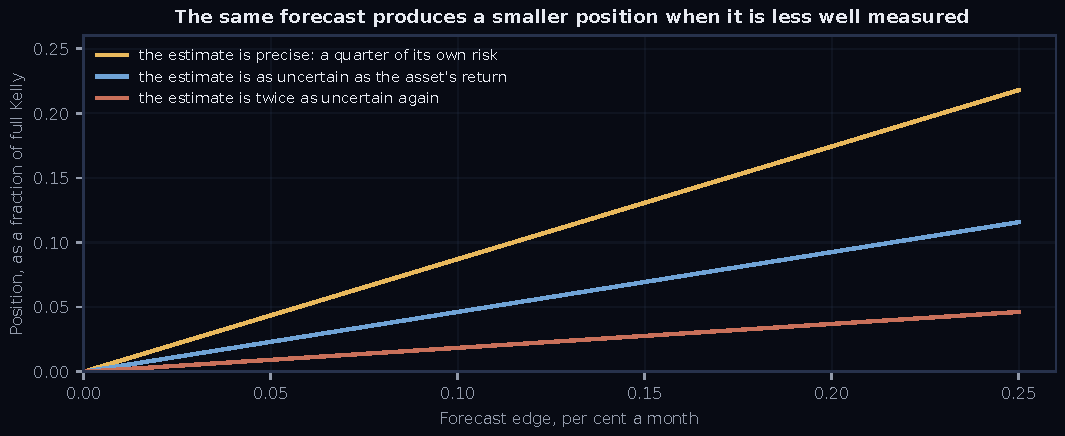
\includegraphics[width=\textwidth]{../figures/fig_kelly_shrinkage.pdf}
\caption{The certainty-equivalent construction. The left panel shows the
distribution of the posterior mean of the edge and its standard
deviation; the right panel shows the resulting position size as a function
of the signal-to-noise ratio of the forecast, against the position size a
naive pipeline would take. The two agree only when the forecast is many
standard deviations from zero.}
\label{fig:kelly-shrinkage}
\end{figure}

\figref{fig:kelly-shrinkage} is the picture the whole book is arguing
for. The right-hand panel is the position size as a function of the
signal-to-noise ratio of the forecast. It rises steeply once the forecast
is a small number of standard deviations from zero, and it is
indistinguishable from zero until then. A naive pipeline holds the
top-ranked names at full weight regardless, and pays the spread on every
trade to find out.

\section{The size of the numbers}

It is worth being concrete, because the reader should know what the
forecasts actually look like.

In this book's data, a representative fund's one-month forward return has
a posterior mean of the order of a tenth of a per cent and a posterior
standard deviation of the order of two to three per cent. The signal to
noise ratio is therefore of the order of 0.05, and the probability that
the edge is positive is about 52 per cent.

That is the honest state of affairs for a price-based model of a liquid
ETF, and it is not a criticism of the model --- it is a statement about
the difficulty of the problem. Chapter 3's evidence says as much from a
different direction. What the model can offer is not certainty but
\emph{calibration}: the probability it reports is a probability, and a
reader who trusts it can size positions against it.

\section{The three ways the posterior can be wrong}

The posterior over the edge can be wrong in three distinct ways, and they
have different remedies.

\textbf{The model is wrong.} The functional form is wrong: the edge is not
a linear function of these twelve features. No amount of calibration
fixes this; the remedy is a better model, and the evidence in Chapter 3
suggests that this is expensive.

\textbf{The posterior is too narrow.} The model does not capture all the
uncertainty --- the uncertainty about the parameters of the model itself,
the uncertainty about which model is right, the uncertainty about whether
the regime has changed. The remedy is the between-model term of Chapter 19
and the discount on the score, both of which widen the posterior when the
evidence is thin.

\textbf{The regime has changed.} The posterior was correct about a
different data-generating process. This is the adaptive-markets case, and
no amount of within-sample care answers it; the remedy is a discount
horizon, a governor, and an acceptance that the record contains one
regime change of a magnitude nobody can predict.

\begin{keytakeaways}
\item The edge is a difference of expected returns, and what the model
produces is a posterior distribution over it, not a number.
\item The probability that the edge is positive is
\(\Phi(\mu/\sqrt{v})\), and for a price-based model of a liquid ETF in
this data that probability is close to one half.
\item A forecast is evidence only when it is many standard deviations from
zero, and the position size must reflect that.
\item The posterior can be wrong because the model is wrong, because the
posterior is too narrow, or because the regime changed; the remedies are
different for each.
\end{keytakeaways}
